\documentclass[a4paper,12pt]{article}
                 
\usepackage[cp1251]{inputenc}  
\usepackage[T2A]{fontenc}      
\usepackage[russian]{babel}
\usepackage{float}
\usepackage{subfigure}

\usepackage{bibtex}
\usepackage{graphicx}

\usepackage{indentfirst}
                 
\usepackage[labelsep=period,labelfont=bf,figurename={Рис.},figurewithin=none]{caption}

\usepackage{wrapfig}

\usepackage{amsmath}

\usepackage{amssymb}

\usepackage[a4paper,top=1.3cm,bottom=2cm,left=1.5cm,right=1.5cm,marginparwidth=0.75cm]{geometry}

\begin{document}                           

\begin{titlepage}
\begin{center}
    {\large МОСКОВСКИЙ ФИЗИКО-ТЕХНИЧЕСКИЙ ИНСТИТУТ (НАЦИОНАЛЬНЫЙ ИССЛЕДОВАТЕЛЬСКИЙ УНИВЕРСИТЕТ)}
\end{center}

\begin{center}
    {\large Физтех-школа радиотехники и компьютерных технологий}
\end{center}

\vspace{3.5cm}

\begin{center}
    
\includegraphics[width=0.4\linewidth]{hv_full.png}
\end{center}

\vspace{0.1cm}

{\huge
\begin{center}
    {\bf Вопрос по выбору}\\
    Закон всемирного тяготения. Точки Лагранжа
\end{center}
}

\vspace{2cm}

\begin{flushright}
{\LARGE Автор:\\ Григорьев Даниил \\
\vspace{0.2cm}
Б01-407}
\end{flushright}

\vspace{3.5cm}
\begin{center}
    Долгопрудный 2025
\end{center}
\end{titlepage}

\section{Введение}

Закон всемирного тяготения, открытый Исааком Ньютоном, описывает силу притяжения между телами, которая зависит от их масс и расстояния между ними.
Этот закон лег в основу понимания движения планет и других небесных тел.
Одним из важных результатов применения этого закона стало открытие точек Лагранжа — особых позиций в гравитационном поле двух крупных объектов,
где маленькие тела могут находиться в стабильном положении.

\section{Законы Кеплера}

В результате длительной обработки многолетних наблюдений датского астронома Тихо Браге (1546-1601) Кеплер (1571-1630) эмпирически установил три закона планетных движений.
Эти законы формулируются следующим образом:

\begin{enumerate}
\item Каждая планета движется по эллипсу, в одном из фокусов которого находится Солнце;
\item Радиус-вектор планеты в равные времена описывает равные площади;
\item Квадраты времен обращений планет относятся как кубы больших осей эллиптических орбит, по которым они движутся вокруг Солнца.
\end{enumerate}                                   

Первые два закона были опубликованы Кеплером в 1609 г., последний В 1619 г. Законы Кеплера естественным путем привели Ньютона к открытию закона всемирного тяготения.
Рассмотрим этот вопрос.

\section{Закон всемирного тяготения}
\subsection{Вывод Ньютона}
Из первого закона Кеплера следует, что траектория планеты плоская кривая. 
С учетом этого обстоятельства\footnote{Это требуется для теоремы: если траектория материальной точки - плоская кривая и радиус-вектор, проведенный из неподвижного полюса О, в равные времена описывает одинаковые площади, то направление действующей силы все время проходит через полюс О.}, из второго закона Кеплера следует, что сила, заставляющая планету двигаться по замкнутым орбитам, направлена к Солнцу. 
Определим теперь, как эта сила изменяется с изменением расстояния от Солнца и как она зависит от массы планеты.
Для упрощения расчетов можно допустить, что планета движется не по эллипсу, а по кругу, в центре которого находится Солнце.
Но я рассмотрю задачу сразу более строго, не прибегая к такому упрощению.

\begin{wrapfigure}{r}{0.3\textwidth}
    \begin{center}
        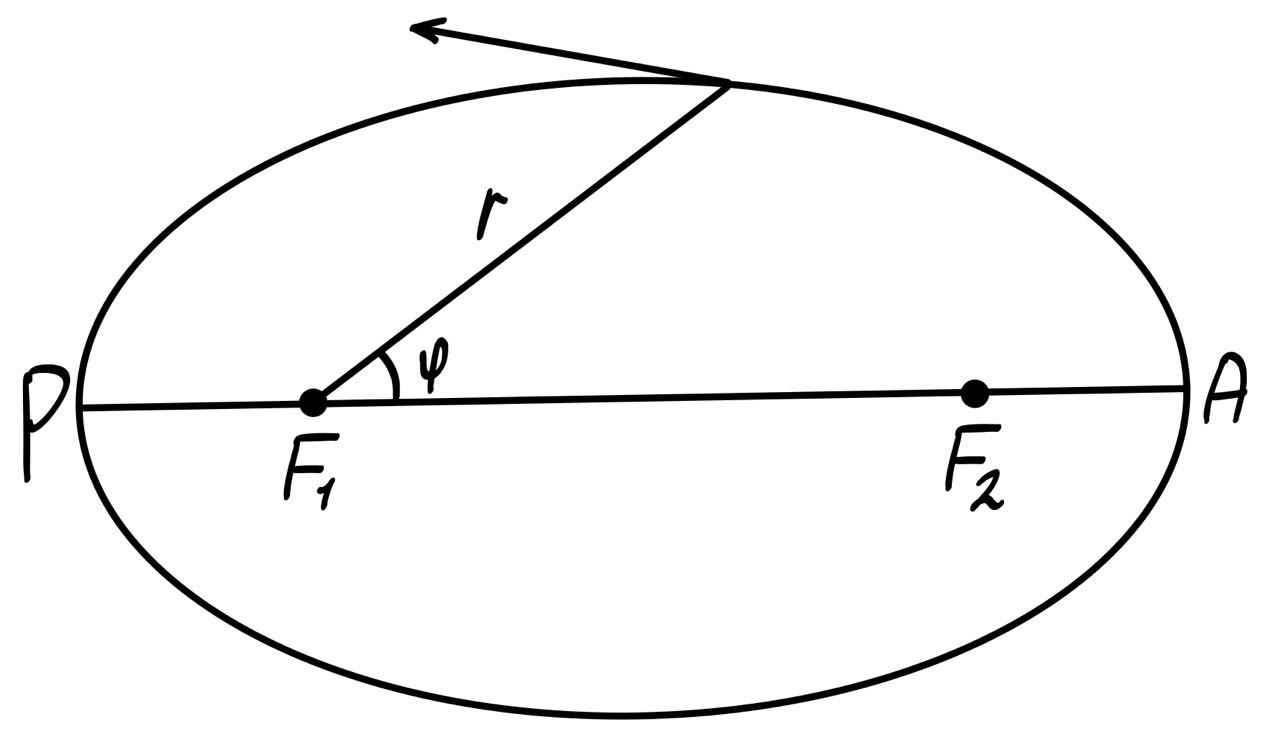
\includegraphics[width=0.3\textwidth]{polar.jpg}
	\caption{Полярная система координат}
    \end{center}
\end{wrapfigure}

Третий закон Кеплера для гиперболических и параболических движений, теряет смысл.
Однако для вычисления ускорения планеты или кометы он и не нужен.

Введём полярную систему координат с полюсом в фокусе $F_1$, где находится Солнце, и полярной осью РА, направленной вдоль большой оси эллипса или гиперболы.

Ускорение движущегося тела разложим на радиальную составляющую $a_r$, направленную вдоль радиуса $r$, и азимутальную составляющую $a_\phi$, перпендикулярную к радиусу.
Они определяются выражениями
$$ a_r = \ddot{r} - \dot{\phi}^2 r, \hspace{25pt} a_\phi = \frac{1}{r} \frac{d}{dt} (r^2 \dot{\phi}) \hspace{25pt} (3.1.1) $$
Величина 
$$ \sigma = \frac{1}{2} r^2 \dot{\phi} \hspace{25pt} (3.1.2) $$
есть секториальная скорость, т. е. площадь, описываемая радиусом-вектором планеты или 
кометы в единицу времени.
По второму закону Кеплера она постоянна, а потому $a_\phi = \frac{1}{r} \frac{d}{dt} (2\sigma)$.
Значит, ускорение рассматриваемого небесного тела не имеет азимутальной составляющей, т.е. направлено к Солнцу.
Производная $\dot{\phi}$ определяется формулой (3.1.2).
Для вычисления производной $\ddot{r}$ воспользуемся уравнением конического сечения в полярной системе координат
$$ r(1 - \epsilon \cos\phi) = p, \hspace{25pt} (3.1.3) $$

где $p$ - параметр эллипса и $\epsilon$ - эксцентриситет. Для эллипса $\epsilon < 1$, для параболы $\epsilon = 1$, для гиперболы $\epsilon > 1$.
В предельных случаях: $\epsilon = 0$ и $\epsilon = \infty$ получаются круг и прямая линия. 
Дифференцируя уравнение (3.1.3) по времени, получим
$$ \dot{r}(1 - \epsilon \cos\phi) + \epsilon r \dot{\phi} \sin\phi = 0, $$
или после умножения на $r$ с учетом соотношений (3.1.2) и (3.1.3) 
$$ p \dot{r} + 2 \epsilon \sigma \sin\phi $$
Вторичное дифференцирование даёт
$$ p \ddot{r} + 2 \sigma \epsilon \cos\phi \dot{\phi} $$
Подставляя сюда  $\dot{\phi} = \frac{2 \sigma}{r^2}, $  $\epsilon \cos\phi = 1 - \frac{p}{r}, $ получим
$$ \ddot{r} = -\frac{4\sigma^2}{pr^2} + \frac{4\sigma^2}{r^3} = -\frac{4\sigma^2}{pr^2} + \dot{\phi}^2 r $$
Из первой формулы (3.1.1) находим 
$$ a_r = -\frac{4\sigma^2}{pr^2}. \hspace{25pt} (3.1.4)$$

Таким образом, ускорение тела обратно пропорционально квадрату её расстояния от Солнца.

Докажем, что коэффициент  $\frac{4\sigma^2}{p}$ один и тот же для всех планет. Площадь эллипса $\pi a b,$ где $a$ и $b$ - длины большой и малой полуосей его.
$\sigma$ - постоянна, тогда $\sigma = \frac{\pi a b}{T},$ где $T$ - период обращения планеты по её орбите. Из аналитической геометрии известно, что $p = \frac{b^2}{a}.$ 
Тогда из (3.1.4)
$$ a_r = -\frac{4\pi^2 a^3}{T^2} \frac{1}{r^2}. \hspace{25pt} (3.1.5)$$
Ввод постоянную Кеплера $K = \frac{a^3}{T^2}$, получим
$$ a_r = -\frac{4\pi^2 K}{r^2}. \hspace{25pt} (3.1.6)$$
Сила, действующая на планету, равна
$$ F = -\frac{4\pi^2 K m}{r^2}. \hspace{25pt} (3.1.7)$$
Коэффициент пропорциональности $4\pi^2 K$, входящий в формулы (3.1.6) и (3.1.7), один и тот же для всех планет, а потому он не может зависеть от массы планеты.
Но Солнце и планета в их взаимодействии выступают как равноправные тела.
Они отличаются друг от друга массами.
И если сила взаимодействия $F$ пропорциональна массе планеты $m$, то она должна быть пропорциональна также и массе Солнца $M$.
Для этой силы можно поэтому написать
$$ F = \gamma \frac{M m}{r^2}. \hspace{25pt} (3.1.8)$$
где $\gamma$ - новая постоянная, уже не зависящая ни от массы Солнца, ни от массы планеты.

Солнце и планеты отличаются друг от друга и от других тел также только количественно величинами масс.
Поэтому естественно предположить, что притяжение существует не только между Солнцем и планетой, но и между планетами,
а также между любыми другими телами, и что сила притяжения определяется формулой (3.1.8), в которой под $M$ и $m$ следует понимать массы взаимодействующих тел.
Это предположение было введено Ньютоном и подтвердилось на опыте. Он сформулировал закон всемирного тяготения,
согласно которому \textit{любые два тела (материальные точки) притягиваются друг к другу с силами,
пропорциональными произведению их масс и обратно пропорциональными квадрату расстояния между ними.}
Такие силы называются гравитационными или силами всемирного тяготения.
Коэффициент пропорциональности $\gamma$, входящий в формулу (3.1.4), один и тот же для всех тел.
В этом смысле он является универсальной постоянной. Это — одна из важнейших мировых постоянных, называемая гравитационной постоянной.
Измерения $\gamma$ современными методами привели к результату
$$ \gamma = (6,6732 \pm 0,0031) \cdot 10^{-8}  \hspace{2pt} dyn \cdot cm^{2} \cdot  g^{-2} 
          = (6,6732 \pm 0,0031) \cdot 10^{-11} \hspace{2pt}   N \cdot  m^{2} \cdot kg^{-2}.$$
Гравитационная постоянная, как мы видим, весьма мала.
Поэтому и гравитационные взаимодействия между обычными телами, даже считающимися большими с общежитейской точки зрения, ничтожно малы.

\subsection{Точки Лагранжа}

\subsubsection{Необходимые условия существования точек Лагранжа}
Для существования точек Лагранжа в системе из двух тел (например, Земля и Луна) необходимо выполнение нескольких условий:
\begin{enumerate}
\item \textit{Гравитационное взаимодействие:} Точки Лагранжа возникают в результате взаимодействия гравитационных сил двух крупных тел.
Это означает, что оба объекта должны обладать массой, достаточной для создания значительного гравитационного поля.
\item \textit{Наличие орбитального движения:} Точки Лагранжа существуют в динамических системах,
где оба тела находятся на орбитах, двигаясь по круговым или эллиптическим траекториям.
Обычно это относится к системам, где оба объекта движутся вокруг общего центра масс.
\item \textit{Устойчивость системы:} Для существования стабильных точек Лагранжа важным условием является наличие баланса между силами гравитационного притяжения и
центробежной силой, возникающей из-за движения тел.
В случае неустойчивых точек Лагранжа небольшие возмущения могут вывести объект из равновесия.
\item \textit{Малые массы третьих тел:} Точки Лагранжа предназначены для малых объектов, масса которых значительно меньше масс двух основных тел.
Эти объекты могут быть спутниками или искусственными спутниками, которые находятся в устойчивом или условно устойчивом положении относительно двух крупных тел.
\end{enumerate}                

\subsubsection{Определение точек Лагранжа}
Точки Лагранжа — это особые положения в системе двух массивных тел, движущихся под действием взаимного тяготения (например, планета и её спутник, звезда и планета),
где третье, существенно менее массивное тело может находиться в равновесии относительно них.
Эти точки являются решениями уравнений движения в системе отсчёта, связанной с массивными телами,
и определяются как положения, где силы притяжения двух тел и центробежная сила, действующая на третье тело, уравновешивают друг друга.
Точки Лагранжа названы в честь французского математика Жозефа-Луи Лагранжа, который исследовал их в XVIII веке в контексте задач небесной механики.
В рамках классической механики существует пять таких точек, обозначаемых $L_1,$ $L_2,$ $L_3,$ $L_4$ и $L_5.$ 

\begin{figure}[H]
    \begin{center}
        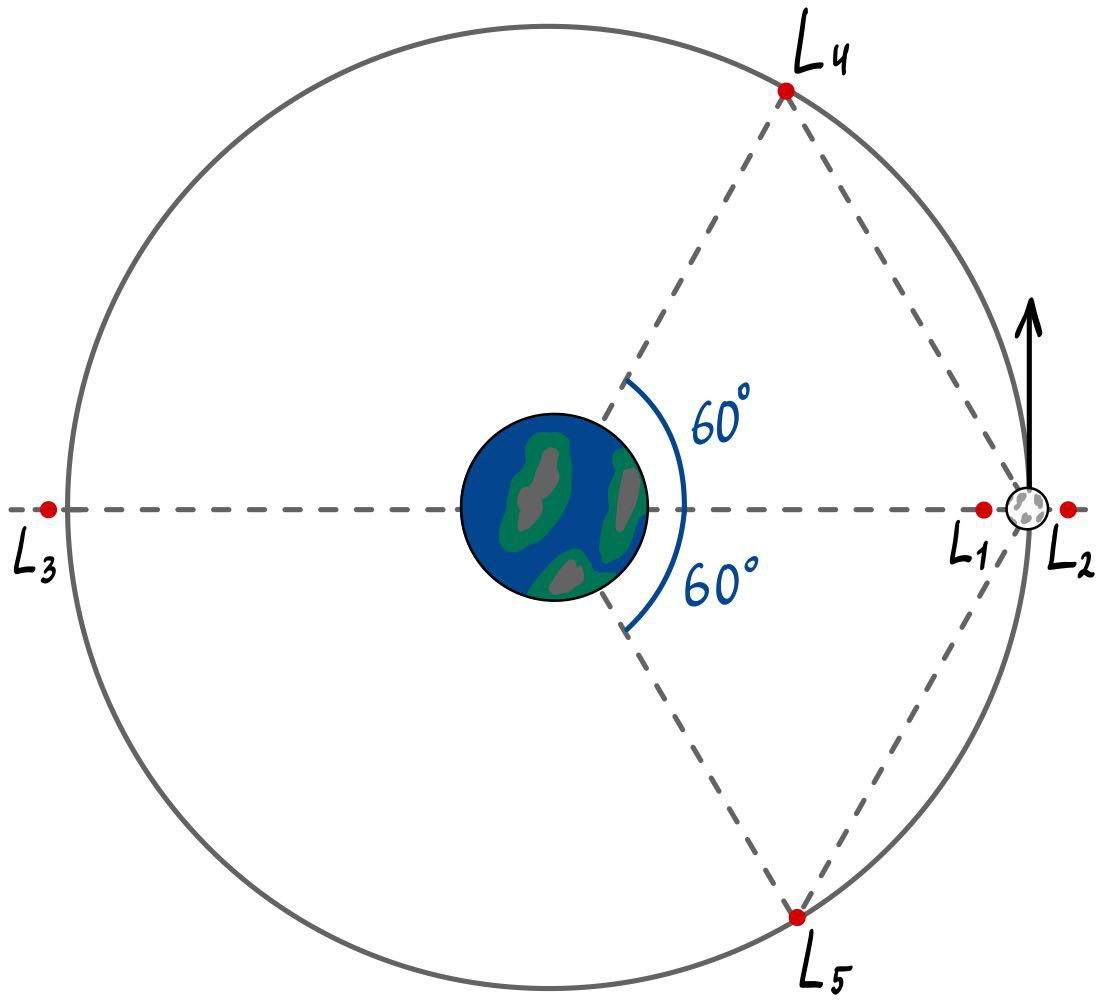
\includegraphics[width=0.6\textwidth]{lagrange.jpg}
        \caption{Точки Лагранжа}
    \end{center}
\end{figure} 
\textit{$L_1:$} Расположена между двумя массивными телами.
Здесь центробежная сила и гравитация уравновешиваются, позволяя менее массивному телу оставаться в этой точке.  \\

\textit{$L_2:$} Находится за меньшим телом (например, за планетой), с внешней стороны относительно большего тела (например, Солнца).
В этой точке силы также компенсируют друг друга. \\

\textit{$L_3:$} Расположена за большим телом на продолжении линии, соединяющей два массивных тела. \\

\textit{$L_4:$} Формирует вершину равностороннего треугольника с двумя массивными телами, находясь на 60° впереди по орбите меньшего тела. \\

\textit{$L_5:$} Аналогичнo $L_4$, но расположена на 60° позади меньшего тела по его орбите. \\

\subsubsection{Точки $L_1$ и $L_2$}

Рассмотрим случай, когда $\vec{r_1}$ $\|$ $\vec{r_2}$ , то есть все три массы лежат на одной прямой.
Пусть пробное тело находится между массивными телами.
Предполагаем, что $l \ll L = r_1 + r_2$, тогда введем обозначение: $l = L\alpha$ где $\alpha \ll 1$
Также, скажем, что $\frac{m_2}{m_1} = \eta$, причем $m_2 \ll m_1$, в ином случае получится
уравнение 5 степени, которое не имеет аналитического решения.                                    
\begin{figure}[H]
    \begin{center}
	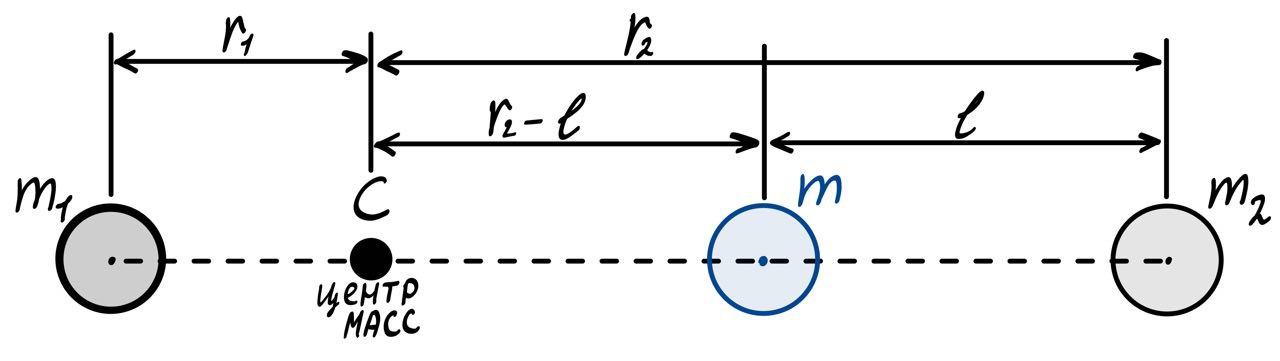
\includegraphics[width=0.6\textwidth]{L1L2.jpg}
	\caption{Картина тел при $\vec{r_1}$ $\|$ $\vec{r_2}$ (Точка $L_1$)}
    \end{center}
\end{figure}
Из определения центра масс 
$$ m_1 r_1 = m_2 r_2  $$
Тогда
$$ r_1 = \eta r_2  $$     
$$ r_2 = \frac{L}{1 + \eta} $$
$$ r_1 = L - r_2 = \frac{\eta L}{1 + \eta}  $$
Таким образом проекции сил, действующих на пробное тело выражаются как
$$ F_1 = -\frac{\gamma m_1 m}{(r_1 + r_2 - l)^2} \hspace{25pt} F_2 = \frac{\gamma m_2 m}{l^2} \hspace{25pt} F_{\omega} = \frac{\gamma (m_1 + m_2) m}{L^3} (r_2 - l) $$
По определению точек Лагранжа
$$ F_1 + F_2 + F_{\omega} = 0 $$
$$ -\frac{\gamma m_1 m}{(r_1 + r_2 - l)^2} + \frac{\gamma m_2 m}{l^2} + \frac{\gamma (m_1 + m_2) m}{L^3} (r_2 - l) = 0 $$
Пользуясь заменами и сокращая, получаем
$$ -\frac{1}{(1 - \alpha)^2} + \frac{\eta}{\alpha^2} + (1 - \alpha - \eta) = 0 $$
Пользуясь тем, что величины малые, а также тем, что $(1 + x)^{\alpha} \approx 1 + x\alpha, x \rightarrow 0$
$$ -(1 + 2\alpha) \alpha^2 + \eta + \alpha^2 - \alpha^3 - \eta \alpha^3 = 0 $$
$$ \alpha^3 (3 + \eta) = \eta  $$
$$ \alpha^3 = \frac{\eta}{3 + \eta} \approx \frac{\eta}{3} $$
$$ \alpha = \sqrt[3]{\frac{\eta}{3}}$$
Окончательно получаем
$$ l = \alpha \cdot L = \sqrt[3]{\frac{m_2}{3 m_1}} L $$
Данная точка - точка $L_1$. Аналогичным образом выводится $L_2$, которая находится справа от тела $m_2$. Формула для неё будет такая же.

\subsubsection{Точка $L_3$}

Теперь рассмотрим ситуацию если пробное тело находится слева от обоих тел
\begin{figure}[H]
    \begin{center}
	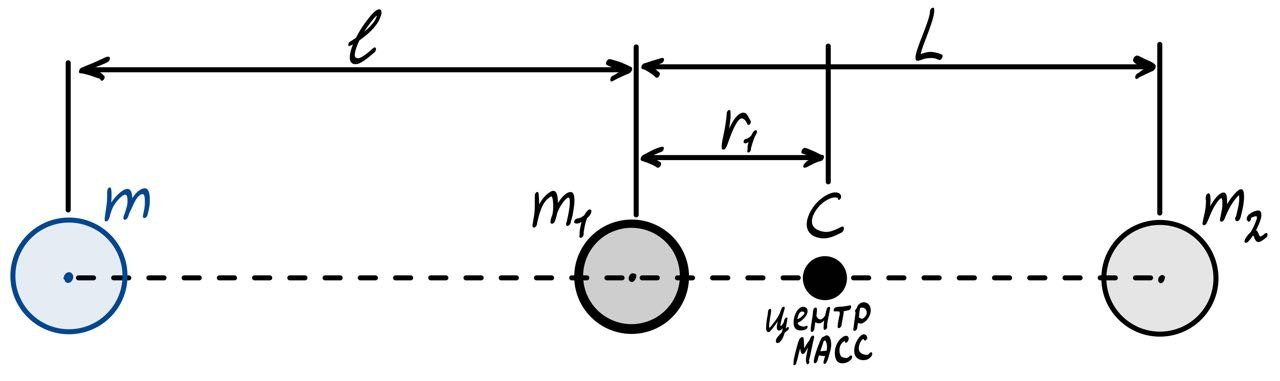
\includegraphics[width=0.6\textwidth]{L3.jpg}
	\caption{Картина тел при $\vec{r_1}$ $\|$ $\vec{r_2}$ (Точка $L_3$)}
    \end{center}
\end{figure}
Тогда уравнение на ускорения примет вид
$$ -\frac{\gamma m_1}{l^2} - \frac{\gamma m_2}{(L + l)^2} + \frac{\gamma (m_1 + m_2)}{L^3} (r_1 + l) = 0 $$
Введем обозначения
$$ l = (1 + \beta) L \hspace{35pt} \frac{m_2}{m_1} = \eta $$
Тогда получаем
$$ r_1 = L - \frac{L}{1 + \eta} = \frac{\eta L}{1 + \eta} $$
$$ l + r_1 = (1 + \beta) L + r_1 = \left(1 + \beta + \frac{\eta}{1 + \eta}\right) L = \frac{1 + \beta \eta + \beta + 2 \eta}{1 + \eta} $$
Тогда
$$ \frac{1}{(1 + \beta)^2 L^2} + \frac{\eta}{(2 + \beta)^2 L^2} - \frac{(1 + \eta)(1 + \beta \eta + \beta + 2 \eta) L}{L^3 (1 + \eta)} = 0 $$
$$ \frac{1}{(1 + \beta)^2} + \frac{\eta}{(2 + \beta)^2} - (1 + \beta \eta + \beta + 2 \eta) = 0 $$
Воспользуемся малостью $\beta$ и получим
$$ 1 - 2 \beta + \frac{\eta}{4}(1 - \beta) - (1 + \beta \eta + \beta + 2 \eta) = 0 $$
$$ \beta = -\frac{7}{12} \eta $$
Таким образом, точка $L_3$
$$ l   = (1 + \beta) L = \left(1 - \frac{7}{12} \eta\right) L $$
$$ l_0 =  l + r_1      = \left(1 + \frac{5}{12} \eta\right) L $$ 

\subsubsection{Точки $L_4$ и $L_5$}

Теперь рассмотрим случай, в котором $\vec{r_1}$ $\nparallel$ $\vec{r_2},$ то есть рассмотрим более общий случай. $m_1$, $m_2$ - рассматриваемые тела, O - положение пробного тела с пренебрежимо малой массой.
C - положение центра масс тел $m_1$ и $m_2$.
Фиксируем линию 1-2, переходя в соответствующую ей вращающуюся систему отсчета

\begin{figure}[H]
    \begin{center}
        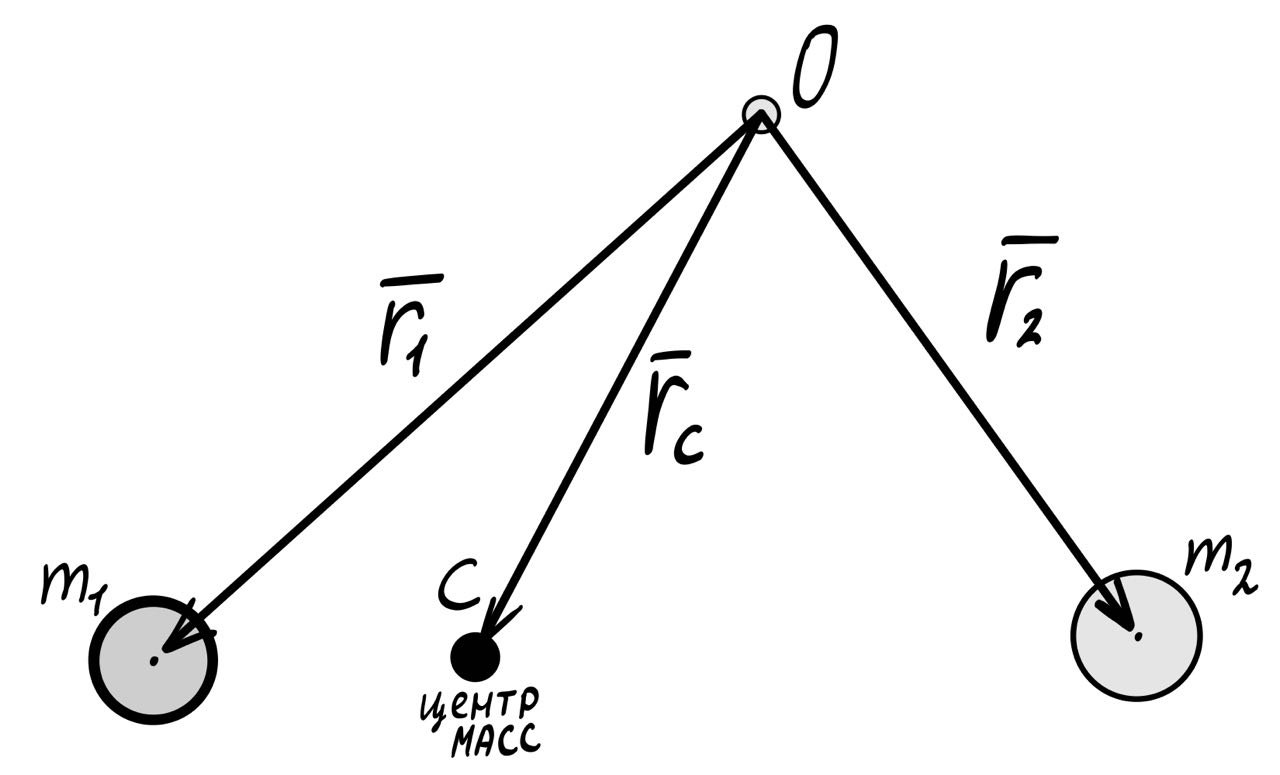
\includegraphics[width=0.6\textwidth]{L4L5.jpg}
	\caption{Картина тел при $\vec{r_1}$ $\nparallel$ $\vec{r_2}$ (Точки $L_4$ и $L_5$)}
    \end{center}
\end{figure}

Ускорение пробного тела
$$ \vec{a} = \frac{\gamma m_1}{r_1^3} \vec{r}_1 + \frac{\gamma m_2}{r_2^3} \vec{r}_2 - \omega^2 \vec{r}_{c}  $$
С учётом $ \omega^2 = \frac{\gamma (m_1 + m_2)}{l^3}, $ где $ l = \left|\vec{r}_1 - \vec{r}_2\right| $ - расстояние между 1 и 2, приобретает вид:
$$ \vec{a} = \gamma m_1 \vec{r}_1 \left(\frac{1}{{r_1}^3} - \frac{1}{l^3}\right) + \gamma m_2 \vec{r}_2 \left(\frac{1}{{r_2}^3} - \frac{1}{l^3}\right) $$
Сделав замену $\xi(r) = \left(\frac{1}{r^3} - \frac{1}{l^3}\right)$, получаем 
$$ \vec{a} = \gamma m_1 \vec{r}_1 \cdot \xi(r_1) + \gamma m_2 \vec{r}_2 \cdot \xi(r_2)  $$
Из определения искомых точек Лагранжа мы знаем что пробное тело должно быть
неподвижным в это СО, а значит его ускорение $\vec{a} = \vec{0}$, тогда:
$$ \vec{a} = \gamma m_1 \vec{r}_1 \cdot \xi(r_1) + \gamma m_2 \vec{r}_2 \cdot \xi(r_2) = \vec{0} \Longleftrightarrow \begin{cases} \xi(r_1) = 0 \\ \xi(r_2) = 0 \end{cases} $$
Так как $\xi(r) = \frac{1}{r^3} - \frac{1}{l^3},$ получаем
$$ r_1 = r_2 = l $$
Этому условию могут удовлетворять только 2 точки, находящиеся в вершинах двух равносторонних треугольниках.
Таким образом мы получили точки Лагранжа - $L_4$ и $L_5$.
                                                                                                  
\subsubsection{Устойчивость точек Лагранжа}

Дело в том, что с точками Лагранжа все-таки есть проблема: $L_1$, $L_2$ и $L_3$ неустойчивы.
Для космического аппарата, помещенного в точку Лагранжа, причин для нарушений точного баланса положения, скорости и сил притяжения – 
хоть отбавляй (притяжение других тел в Солнечной системе оказывает воздействие, орбиты отличаются от круговых, 
скорость оказывается не идеально точной для пребывания в точке Лагранжа и т.д.).
В результате аппарат начинает удаляться от математически определенной точки Лагранжа.
Неустойчивость означает, что по мере сползания на космический аппарат действуют силы, уводящие его только дальше.
Поэтому начавшееся по любой причине сползание не исправится само;
если там оказался астероид, то он со временем сдвинется куда-то прочь.
Линеаризация уравнений движения показывает, что отклонения от этих точек растут экспоненциально, что доказывает их неустойчивость.
А если мы желаем, чтобы там оставалось какое-то устройство, то потребуются включения корректирующего двигателя.
Да, некоторое количество топлива тратится, но очень небольшое – именно из-за того, что дело происходит вблизи точки равновесия
с достаточно вяло проявляющей себя неустойчивостью.
Космический аппарат, который время от времени заботится о своем положении, может поэтому описывать вокруг точки Лагранжа
что-то вроде орбиты, но это орбита не в кеплеровском смысле, поскольку в сторону самой
точки Лагранжа нет силы притяжения, а скорее контролируемый дрейф – сначала сползание
в одну сторону, затем короткое включение двигателя для изменения направления движения,
спутник летал вокруг $L_2$ по такой орбите, чтобы Луна не загораживала ему вид на Землю. При
взгляде с Земли эта орбита проходит снаружи от лунного диска, нигде не заходя за него, – как
«гало» вокруг Луны. Поэтому такие орбиты иногда называют гало-орбитами.

Если говорить про систему Солнце-Земля, то окрестности точки $L_2$ оказываются идеальной «движущейся парковкой» – площадкой для астрономических наблюдений. Эта точка
Лагранжа расположена на расстоянии 1,5 млн км от Земли – что в сто раз меньше расстояния
от Земли до Солнца, но все же в четыре раза дальше, чем находится от нас Луна. Именно
из $L_2$ системы Солнце – Земля изучали реликтовое излучение (космический микроволновой
фон) аппараты WMAP и «Планк». Относительно недавно там же поселился и «Спектр-РГ» –
российско-германская астрофизическая обсерватория; аппарат, запущенный в июле 2019 г., за
100 дней добрался до окрестностей $L_2$, а к середине апреля 2020 г. выполнил один оборот по
орбите, которая проходит на расстоянии до 400 000 км от $L_2$, перпендикулярно линии Солнце –
Земля (рис. ). Контроль за дрейфом в сторону от точки Лагранжа требует краткосрочных включений двигателя каждые 40–70 дней.
В результате космический аппарат будет делать чтото вроде полного оборота в течение примерно полугода, поднимаясь над плоскостью земной
орбиты и опускаясь под нее; траектория образует не очень аккуратный «моток» вокруг $L_2$, мало
похожий на строгий и совершенный эллипс.
\begin{figure}[H]
    \begin{center}
        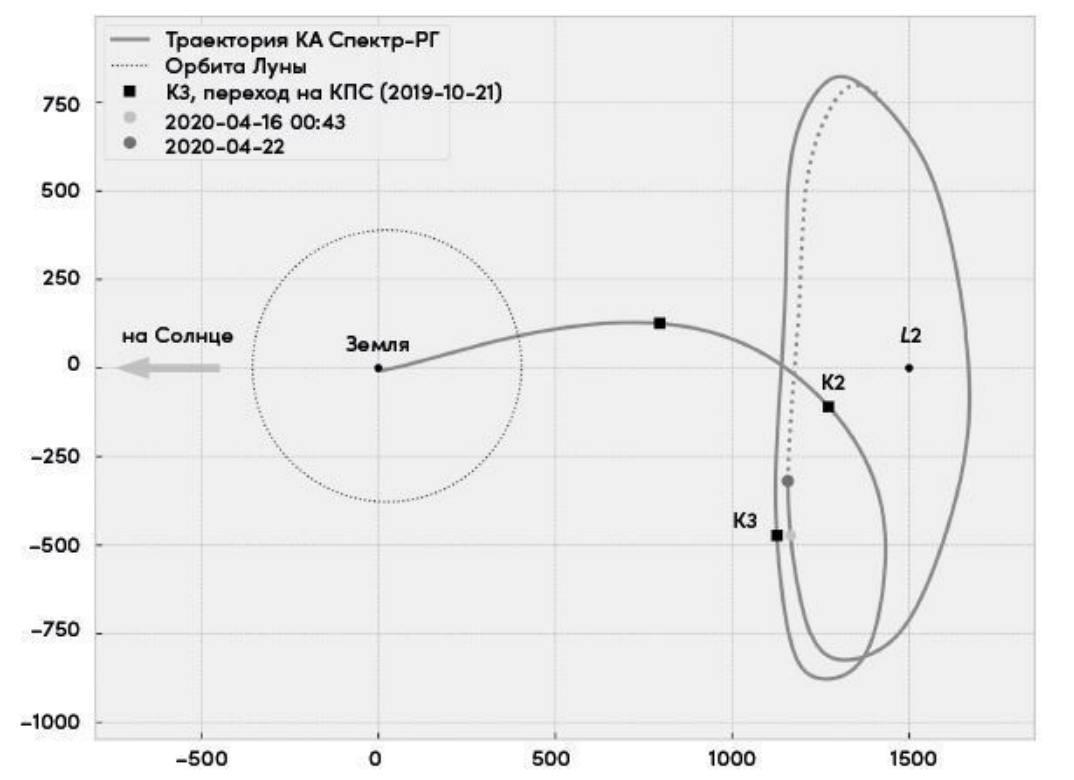
\includegraphics[width=0.6\textwidth]{spektrG.jpg}
	\caption{Траектория аппарата «Спектр-РГ», работающего вблизи точки Лагранжа $L_2$
системы Солнце – Земля, данные ИПМ им. М. В. Келдыша РАН}
    \end{center}
\end{figure}
В точках $L_4$ и $L_5$, например, собираются астероиды, потому что там иная картина с устойчивостью, чем в трех других точках Лагранжа.
С первого взгляда, ситуация даже хуже, потому что баланс сил притяжения таков, что при выходе из точки Лагранжа
в любом направлении возникает сила, которая побуждает уходить дальше.
Кроме притяжения, в дело вступает движение.
Сама точка Лагранжа движется по окружности, а в этом случае есть вот какая новость:
при движении относительно вращающейся системы тело испытывает действие силы Кориолиса.
По мере удаления от $L_4$ уходящее тело набирает скорость относительно этой точки Лагранжа.
Но, поскольку все происходит во вращающейся системе, движущееся
тело испытывает дополнительное воздействие по мере набора скорости.
Баланс всех факторов в окрестности $L_4$ таков, что при развитии сползания тело не уходит прочь,
а, набрав некоторую скорость, отправляется по орбите вокруг точки $L_4$.
Все то же самое происходит и в окрестности $L_5$. Точки $L_4$ и $L_5$ оказываются устойчивыми, если
более массивное из двух больших тел тяжелее другого в $\frac{25 + 3 \sqrt{69}}{2} = 24.95993...$ раза или больше
(с доказательством этого факта можно ознакомиться из \cite{Neil} номера из списка литературы, я его не рассматриваю из-за большого обьема).
Это условие выполнено для пары Земля – Луна и с большим запасом выполнено для всех пар Солнце – планета.

\section{Явления, связанные с точками Лагранжа}

\subsection{Полость Роша}

\textit{Полость Роша} — область вокруг звезды в двойной системе, границей которой служит эквипотенциальная поверхность, содержащая первую точку Лагранжа $L_1.$
В системе координат, вращающейся вместе с двойной звездой, для пробного тела, находящегося в этой области,
притяжение звезды, находящейся в полости Роша, преобладает и над притяжением звезды-компаньона, и над центробежной силой.

В точке Лагранжа $L_1$ полости Роша компонентов двойной системы соприкасаются: равнодействующая притяжений обеих звёзд обращается в ней в нуль.
Это приводит к возможности перетекания вещества от одной звезды к другой при заполнении одной из них полости Роша в ходе её эволюции.
Такие перетекания играют важную роль при эволюции тесных двойных звёздных систем.
\begin{figure}[H]
    \begin{center}
	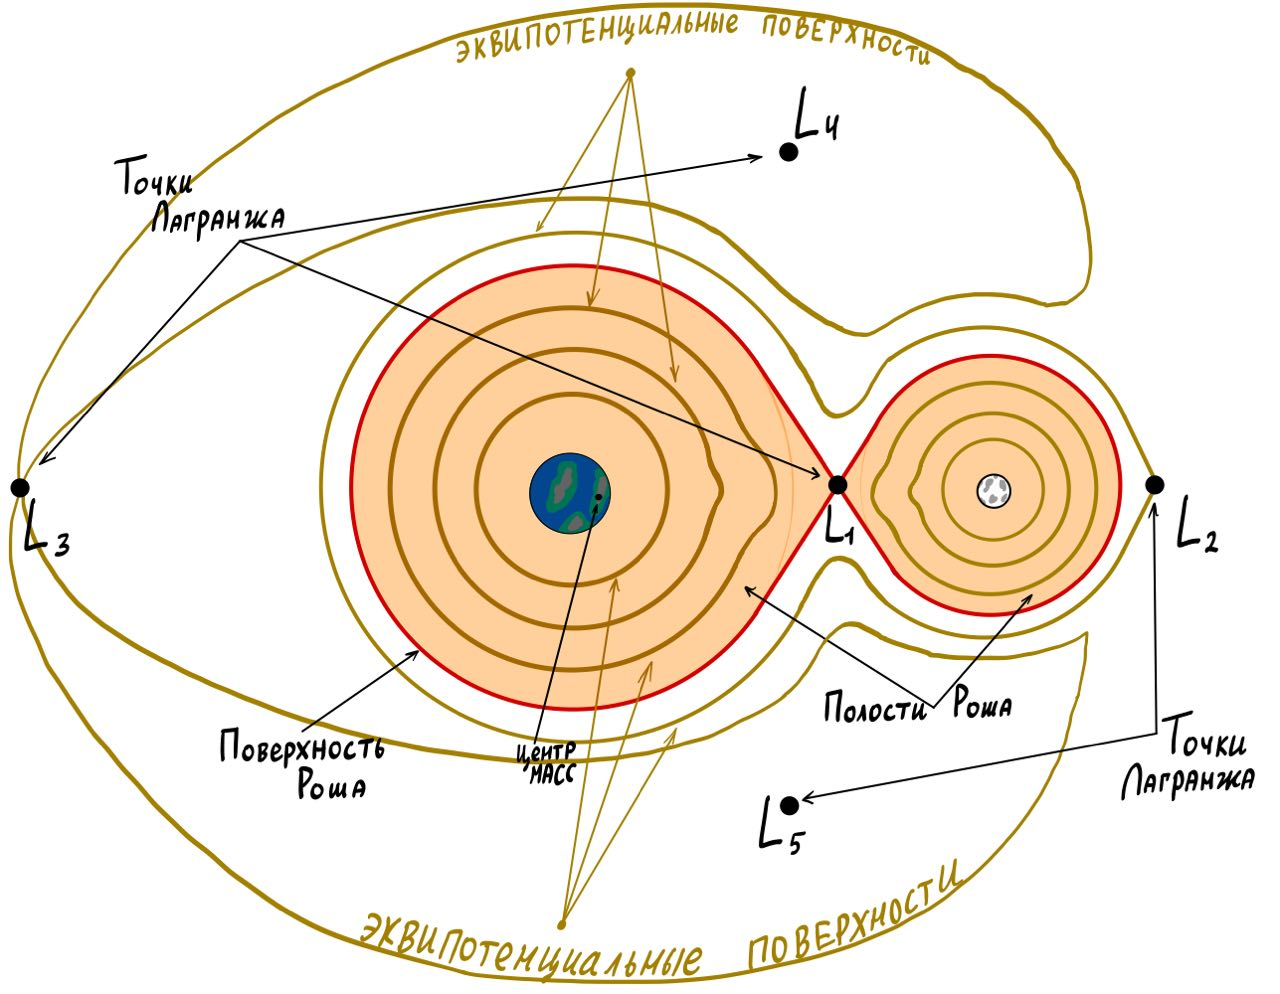
\includegraphics[width=0.6\textwidth]{roche.jpg}
	\caption{Полости Роша для двойной системы}
    \end{center}
\end{figure}
Питером Эгглтоном предложена эмпирическая формула для радиуса полости Роша (радиус шара, объём которого равен объёму соответствующей полости Роша),
дающая результаты с точностью лучше $1\%$ во всём диапазоне отношения масс:
$$ \frac{R_{L}}{a} = \frac {0.49 q^{2/3}}{0.6 q^{2/3} + \ln{(1+q^{1/3})}},\quad 0 < q < \infty, $$
где 
$ R_{L} $ — радиус Полости Роша для звезды с массой $M_1$, 
$  a    $ — большая полуось орбиты (расстояние между центрами масс двух объектов),
$ q = \frac{M_{2}}{M_{1}} $ —  отношение масс звезды ($M_1$) и её компаньона ($M_2$).

\subsection{Сфера Хилла}

\textit{Сфера Хилла} — в первом приближении — пространство вокруг астрономического объекта (например, планеты), в котором он способен удерживать свой спутник,
несмотря на притяжение объекта, вокруг которого обращается сам (например, звезды).
В свою очередь, у спутника есть собственная сфера Хилла, и любой объект в её пределах будет стремиться стать спутником спутника, а не планеты.
Таким образом, сфера Хилла описывает сферу гравитационного влияния тела на более мелкие тела с учётом пертурбаций, возникающих под воздействием более массивного тела.
\begin{figure}[H]
    \begin{center}
	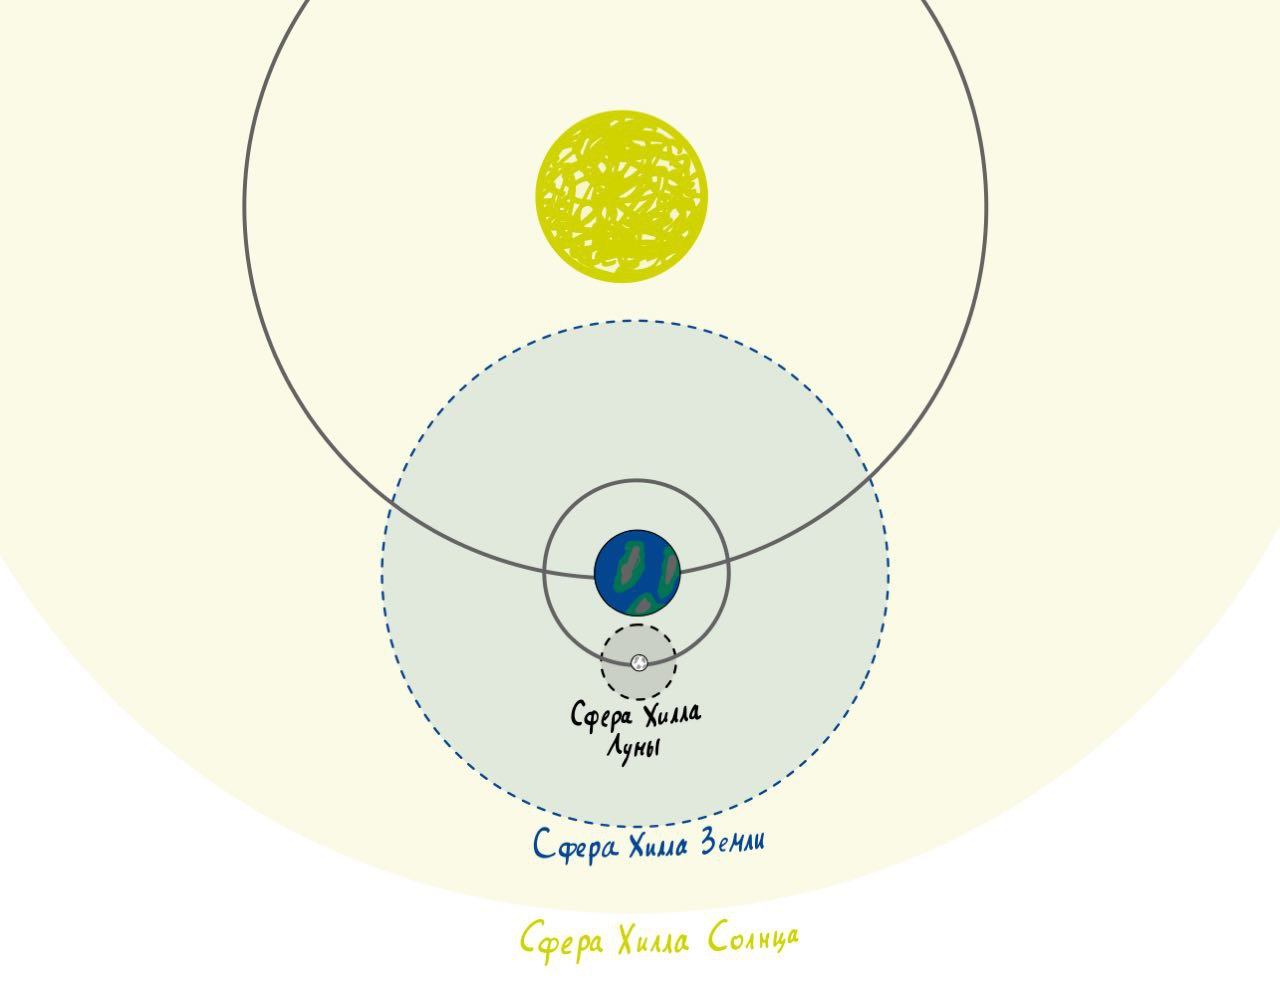
\includegraphics[width=0.6\textwidth]{Hill.jpg}
	\caption{Сферы Хилла для системы Солнце-Земля-Луна}
    \end{center}
\end{figure}
Сфера Хилла располагается между точками Лагранжа $L_1$ и $L_2$, лежащими на прямой, соединяющей центры двух тел.
В этом направлении область гравитационного влияния подчинённого тела меньше всего, и это ограничивает размер сферы Хилла.
За пределами этого расстояния орбита любого третьего тела, обращающегося вокруг подчинённого тела, будет частично пролегать за пределами сферы Хилла,
и поэтому будет всё больше и больше подвергаться возмущению приливными силами центрального тела.
В конечном итоге подчинённый объект перейдёт на орбиту центрального тела.
Для двух тел массами $m$ и $M$ ($m \ll M$) радиус сферы Хилла рассчитывается следующим образом:
$$ r \approx a \sqrt[3]{\frac{m}{3M}}, $$ где $a$ - большая полуось орбиты менее массивного тела.

\section{Модель}

Для наглядности я решил написать две программы на языке программирования С++. В первой программе мы ``сидим`` во вращательной системе отсчета Земля-Луна.
В каждой точке пространства можно узнать векторы действующих сил, просто поставив на это место курсор.
По нажатии левой кнопки мыши в этой точке появится комета массой 100 кг. Тёмно-синими точками нарисованы точки Лагранжа.   

\begin{figure}[H]
    \centering
    \subfigure[Написанная программа, модель]{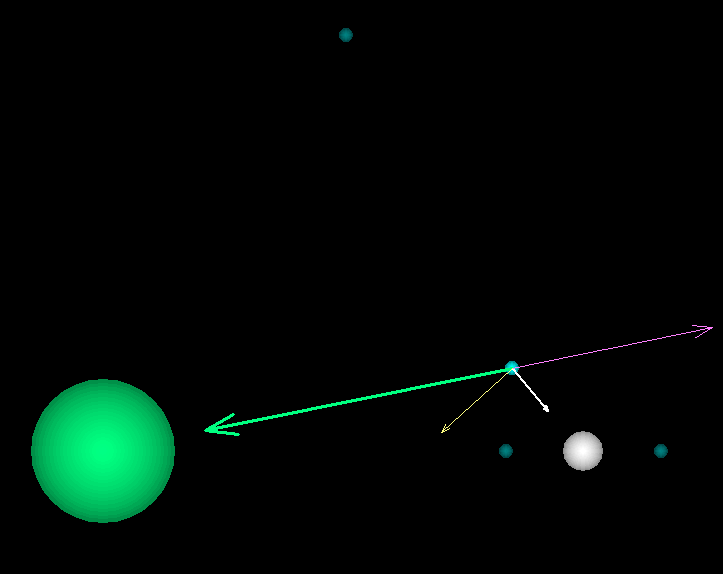
\includegraphics[width=0.4\textwidth]{forces.png}} 
    \subfigure[Схема сил, пояснение модели]{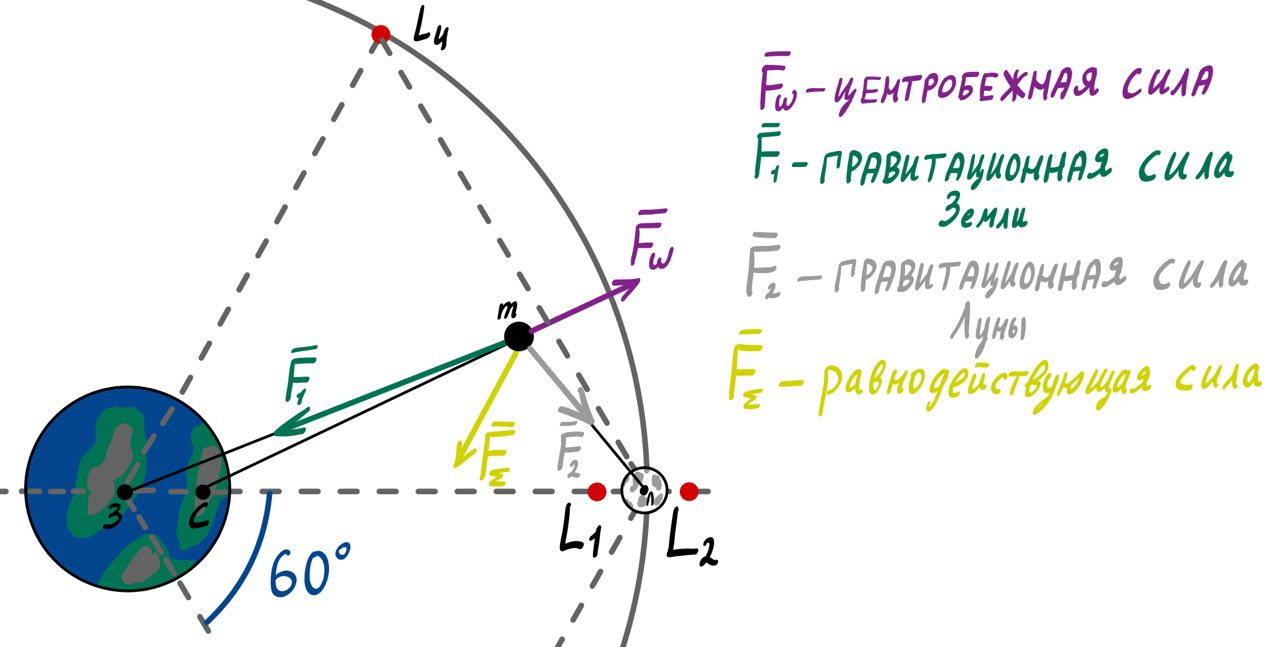
\includegraphics[width=0.4\textwidth]{forcespic.jpg}}
    \caption{Силы, действующие на комету в системе Земля-Луна}
    \label{}
\end{figure}

С помощью данной программы легко увидеть, в каких точках системы модуль равнодействующей силы находится около нулевого значения. Также, есть возможность "запускать"
комету, задавая ей скорость зажатой левой кнопкой мыши.  
\begin{figure}[H]
    \begin{center}
	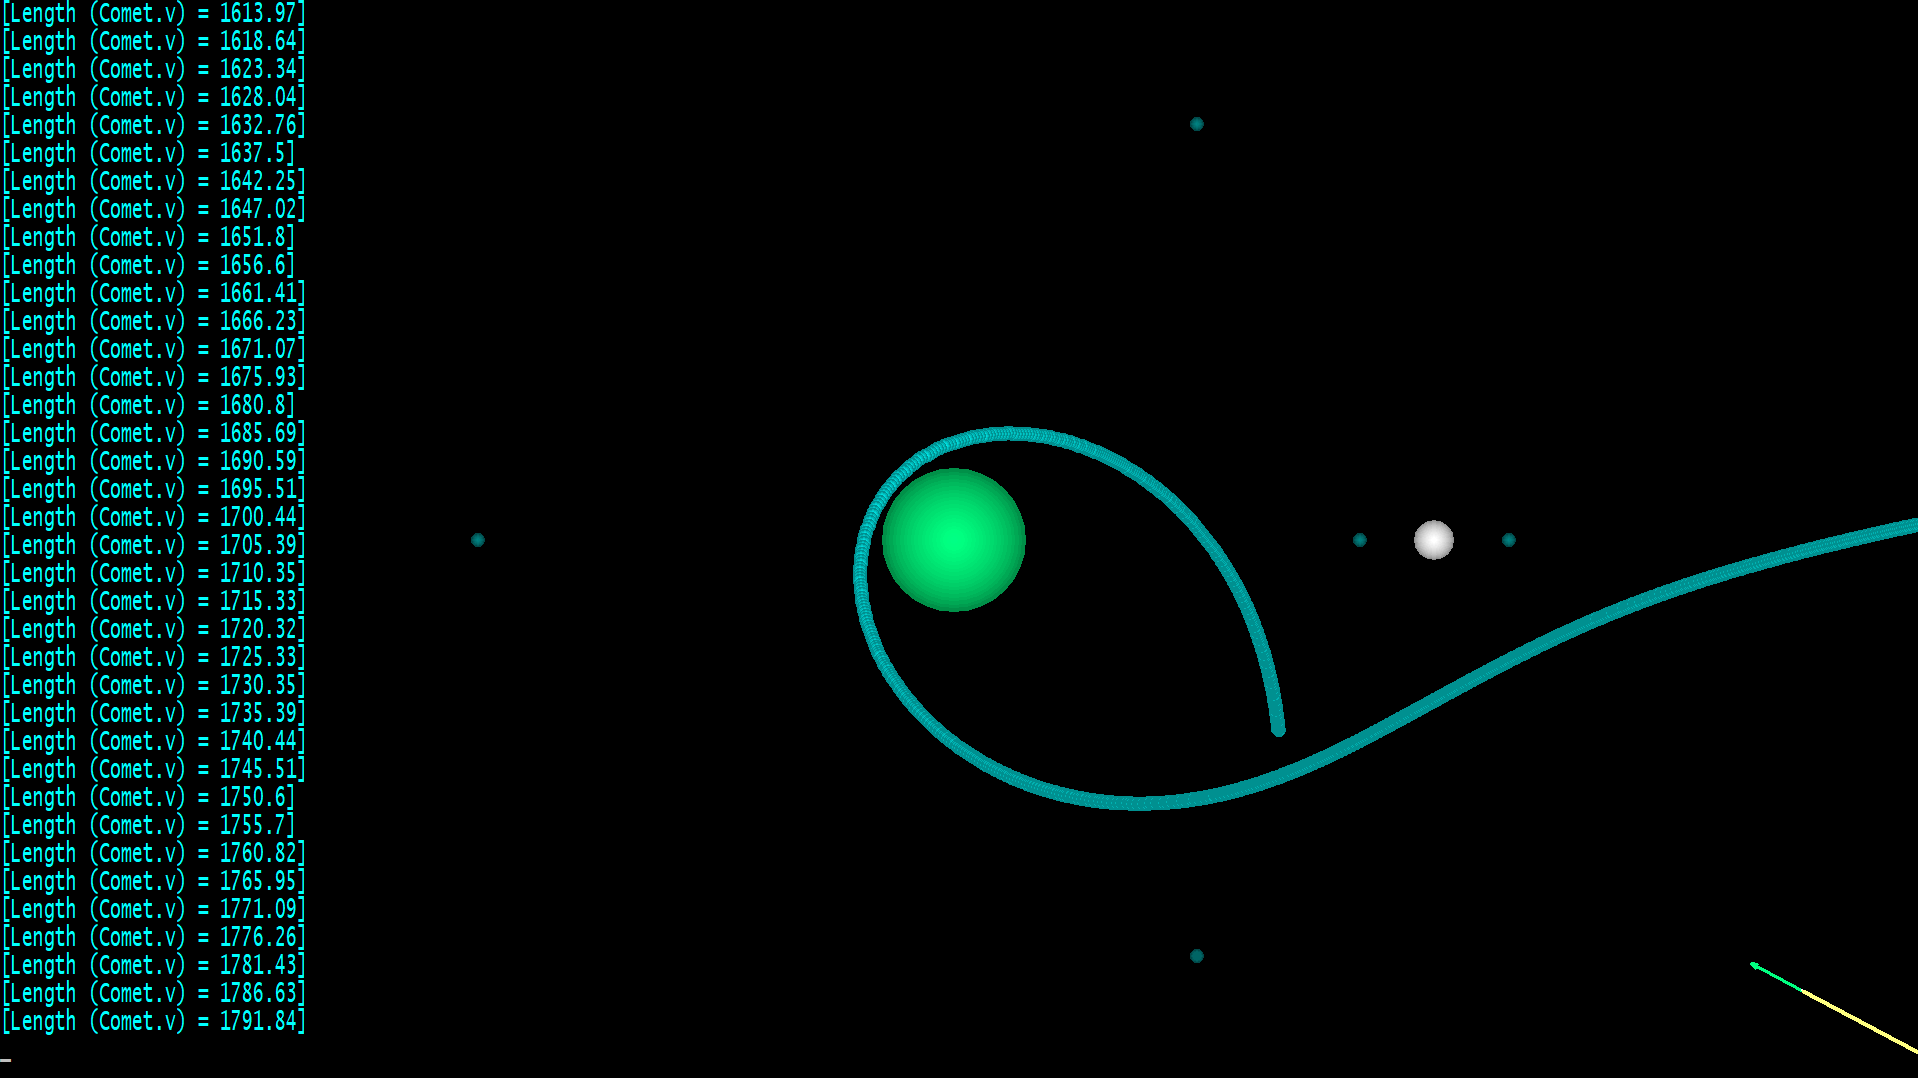
\includegraphics[width=0.8\textwidth]{example_1.png}
	\caption{Пример запуска кометы в случайном направлении во вращательной системе отсчёта. Синия линия - траектория кометы}
    \end{center}
\end{figure}

Вторая программа показывает вращение системы Земля-Луна относительно их общего центра масс. Здесь также отмечены точки Лагранжа и есть возможность запуска кометы.
\begin{figure}[H]
    \begin{center}
	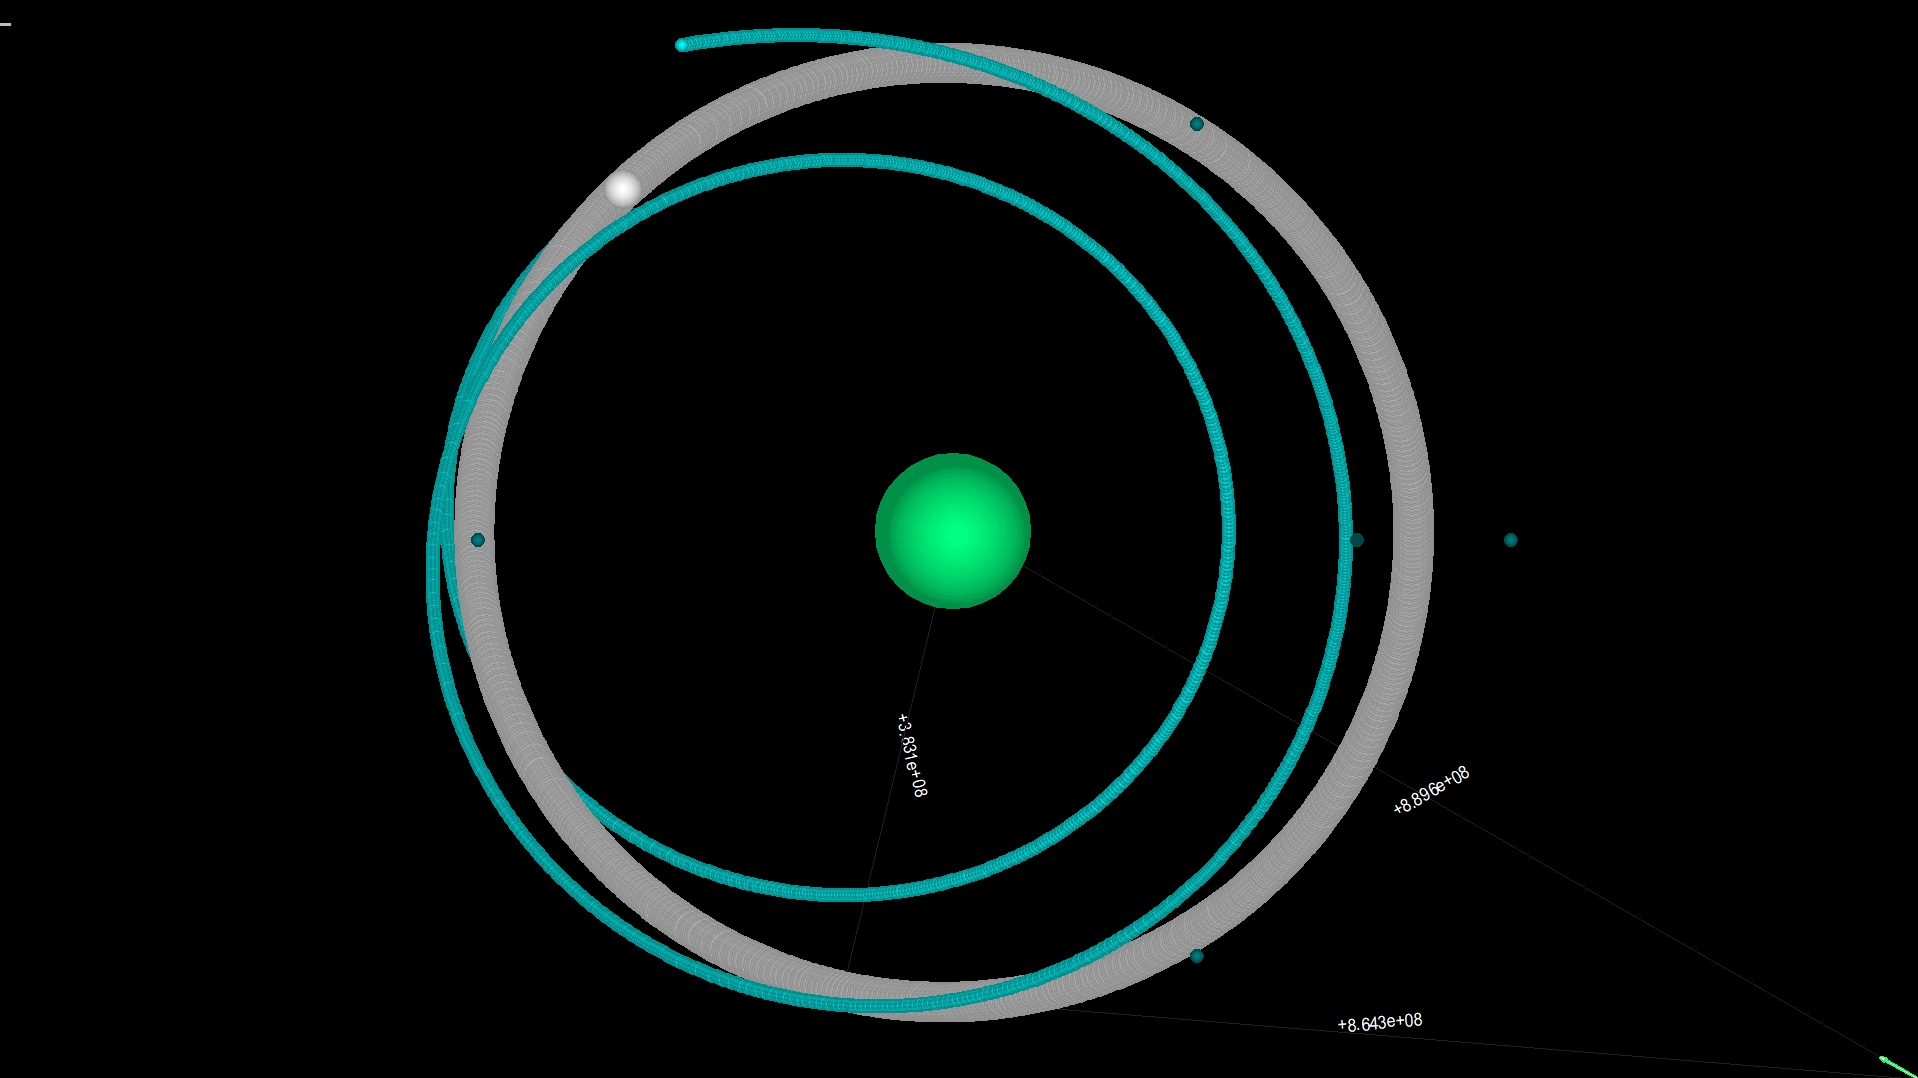
\includegraphics[width=0.8\textwidth]{example_2.png}
	\caption{Пример запуска кометы в случайном направлении. Синия линия - траектория кометы, белая - траектория Луны}
    \end{center}
\end{figure}

Разместим, желтую комету в точке Лагранжа, допустим, в $L_5$ во вращательной системе отсчета. И мы видим, что комета стоит и не двигается! Но это лишь первое время. 
По распечатке слева, видно, что скорость кометы медленно растет. Это происходит из-за того, что на комету действует какая-то малая равнодействующая сила,
которая хоть и медленно, но стаскивает комету с точки Лагранжа.
\begin{figure}[H]
    \begin{center}
	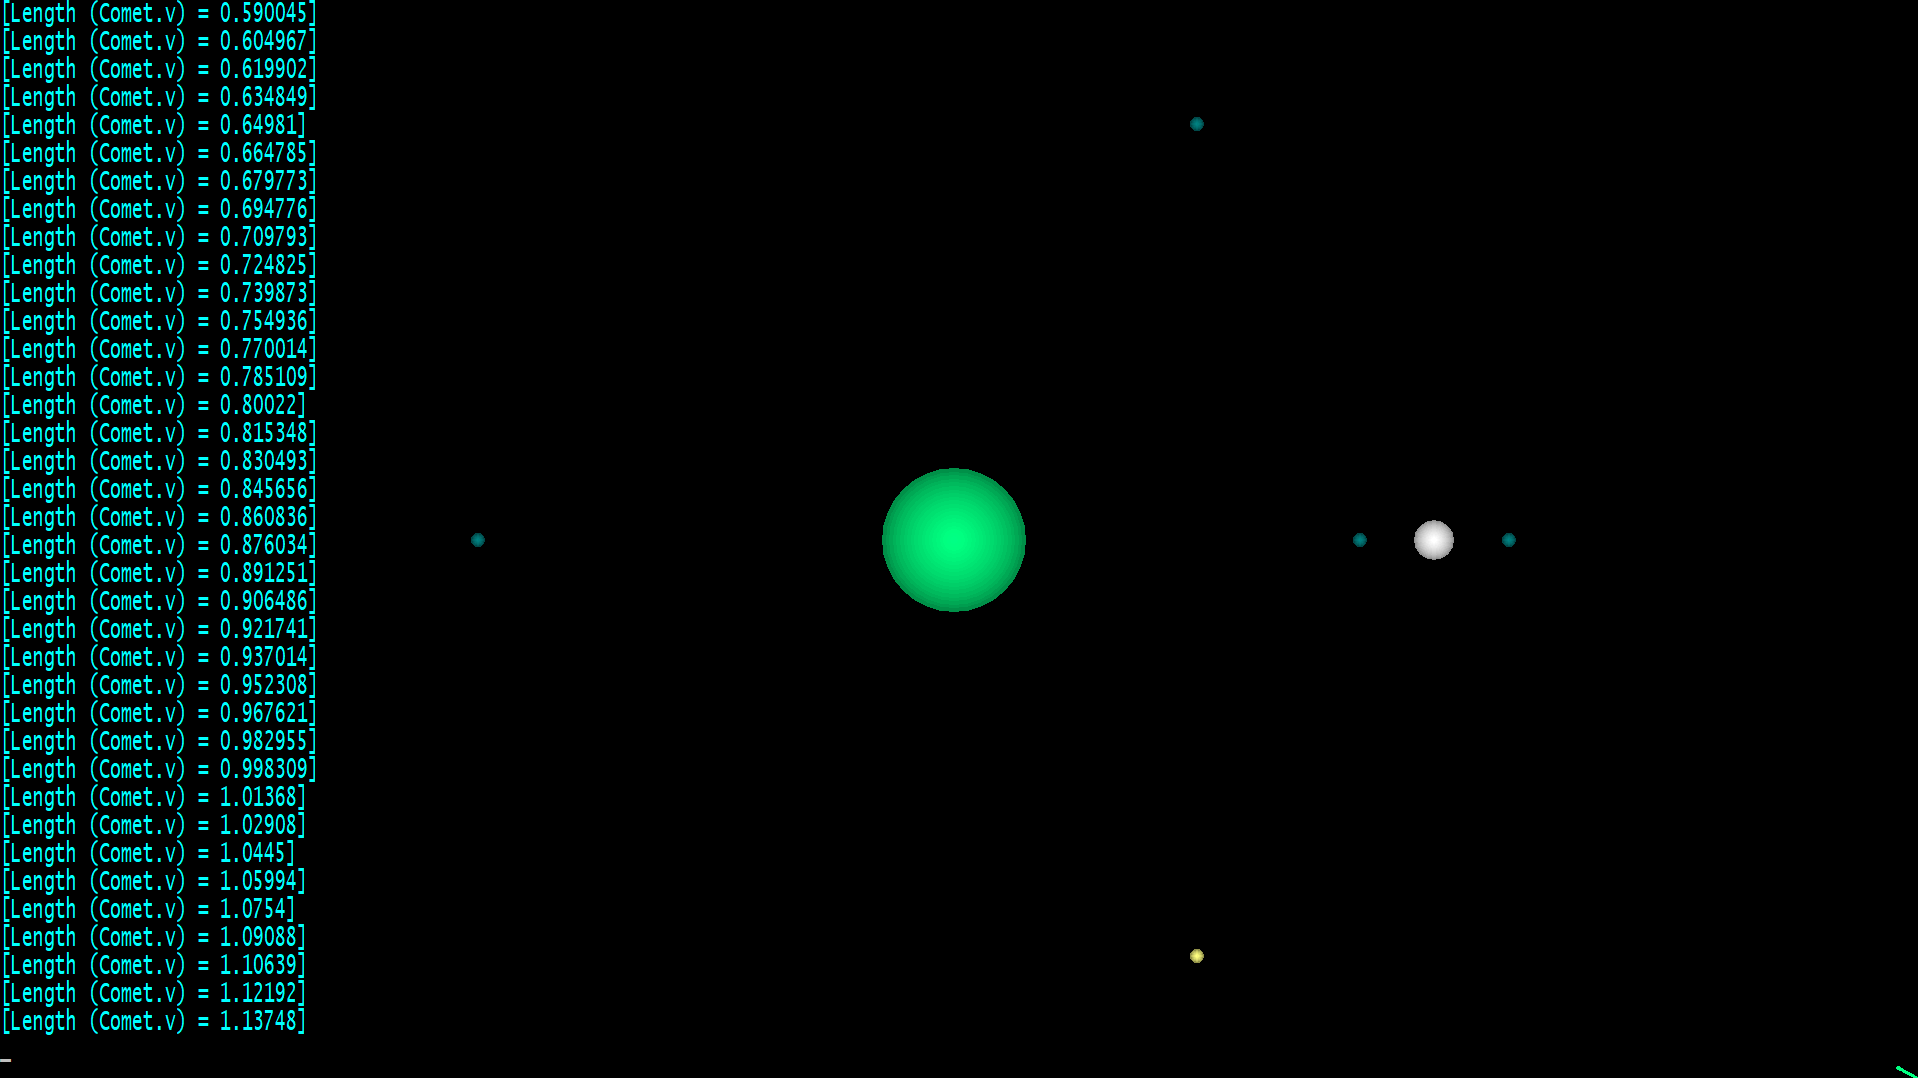
\includegraphics[width=0.8\textwidth]{example_3.png}
	\caption{Комета в точке $L_5$}
    \end{center}
\end{figure}

В промежуточной версии одной из программ удалось сделать схему, на которой показано как меняется результирующая сила на комету в зависимости от её расположения.
\begin{figure}[H]
    \begin{center}
	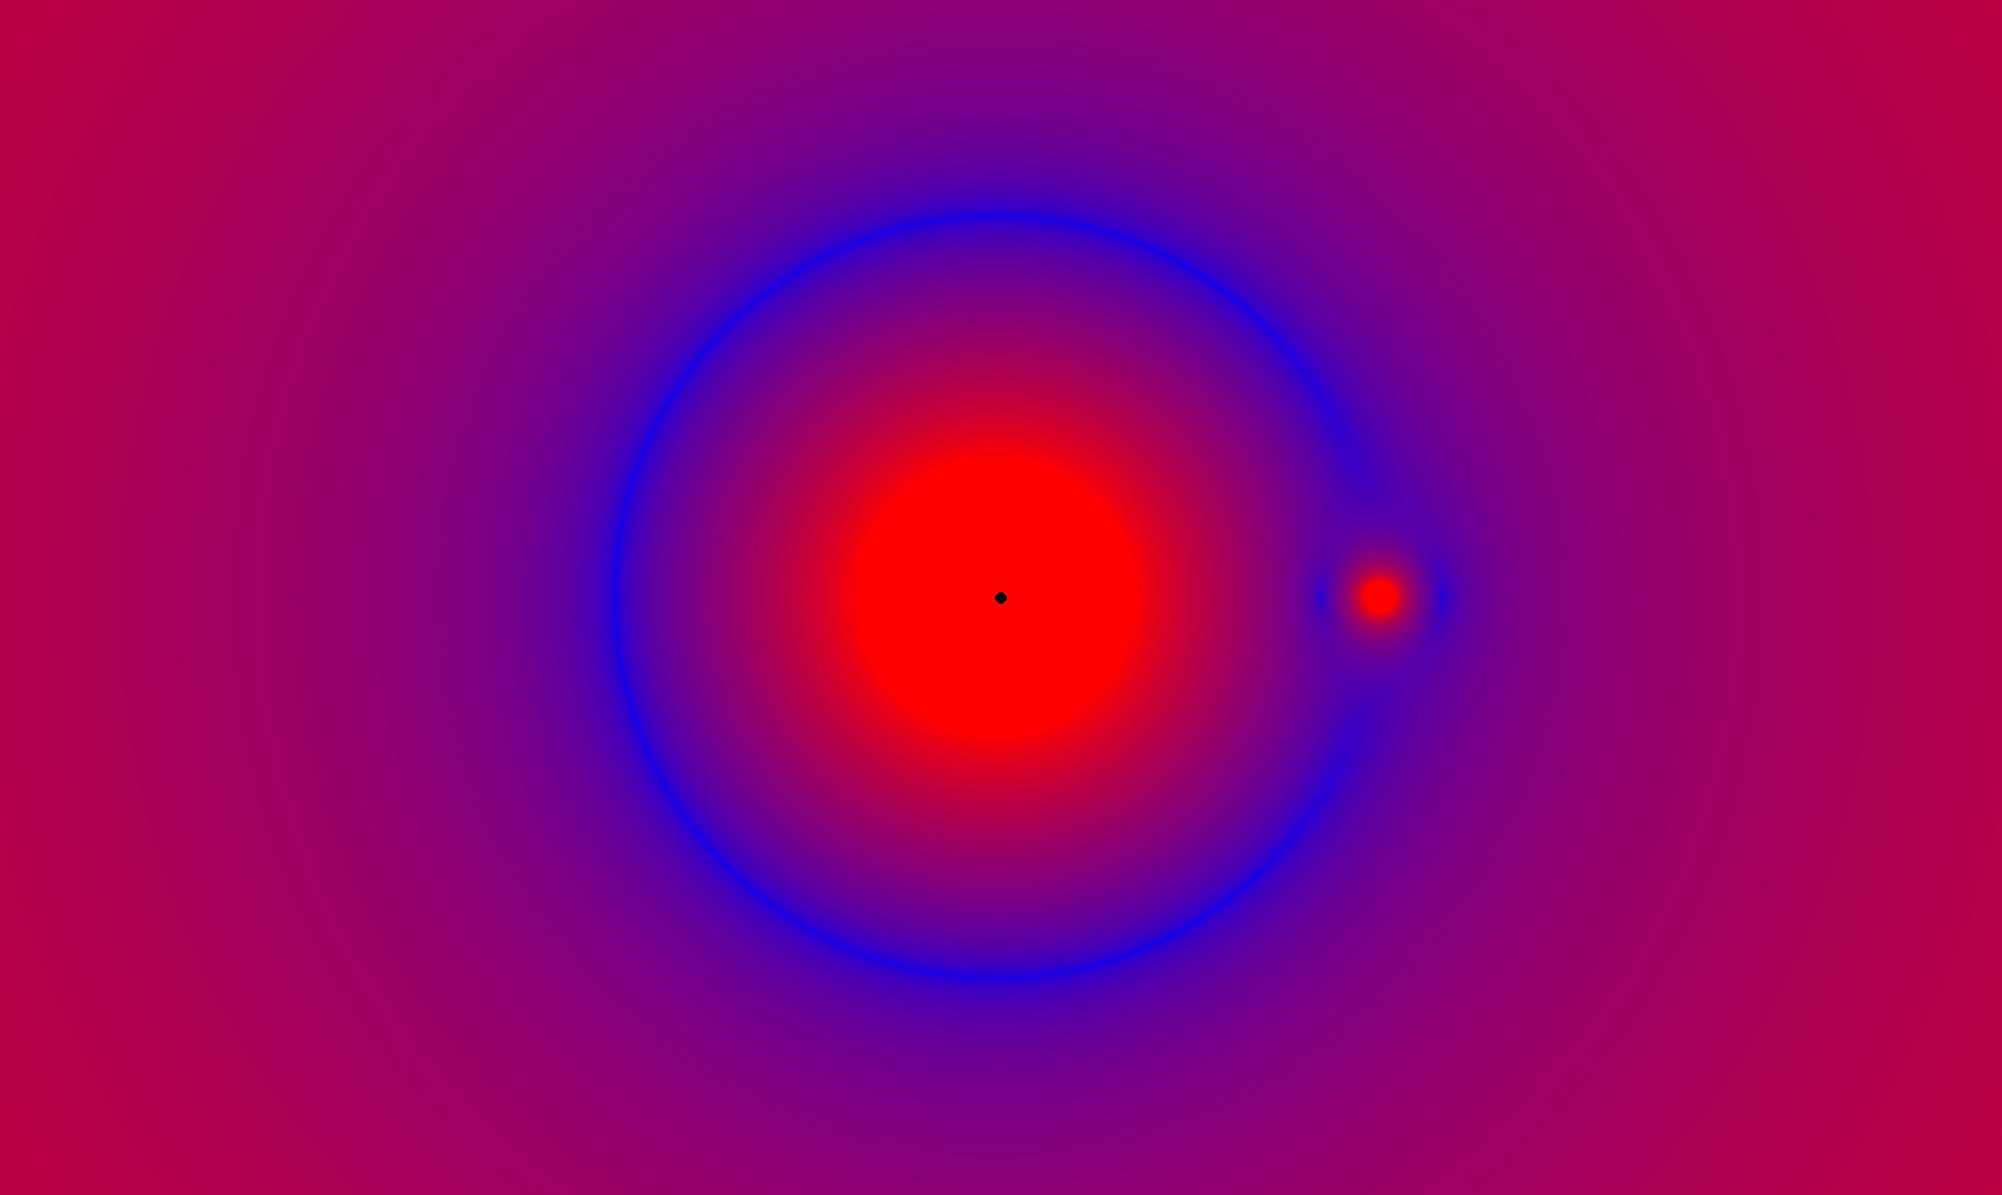
\includegraphics[width=0.8\textwidth]{resultforce.jpg}
	\caption{Красный цвет отвечает за большие значения результирующей силы, синий - за малые}
    \end{center}
\end{figure}

\section{Применение точек Лагранжа}

\subsection{Точкa $L_1$}

Точка $L_1$ находится между Землёй и Солнцем, примерно в $1.5*10^6$км от Земли. Это идеальное место для наблюдения за Солнцем и космической погодой,
так как обсерватории здесь могут получать непрерывный поток данных о солнечном ветре и солнечной активности.

\begin{enumerate}

\item \textbf{SOHO (Solar and Heliospheric Observatory)}

Запущен в 1995 году совместно ESA и NASA.

Основные задачи:
\begin{itemize}
\item Наблюдение за солнечной активностью.
\item Исследование солнечного ветра и короны.
\end{itemize}
Достижения:
\begin{itemize}
\item Впервые обеспечил непрерывное наблюдение за Солнцем в реальном времени.
\item Обнаружил тысячи комет.
\end{itemize}

\item \textbf{ACE (Advanced Composition Explorer)}

Запущен в 1997 году NASA.

Основные задачи:
\begin{itemize}
\item Изучение потоков солнечного и межзвёздного излучения.
\item Мониторинг космической погоды.
\end{itemize}
Достижения:
\begin{itemize}
\item Помог предсказывать солнечные вспышки, влияющие на спутники и энергосистемы на Земле.
\end{itemize}

\item \textbf{DSCOVR (Deep Space Climate Observatory)}

Запущен в 2015 году NASA.

Основные задачи:
\begin{itemize}
\item Мониторинг солнечного ветра для прогнозирования космической погоды.
\item Наблюдение за Землёй (например, глобальные климатические изменения).
\end{itemize}
Достижения:
\begin{itemize}
\item Мониторинг космической погоды.
\item Наблюдение за Землёй.
\end{itemize}

\end{enumerate}

\subsection{Точка $L_2$}

\begin{enumerate}

\item \textbf{Телескоп Джеймса Уэбба (JWST)}
                                         
Запущен в декабре 2021 года NASA, ESA и CSA.

Основные задачи:
\begin{itemize}
\item Изучение формирования звёзд и галактик.
\item Исследование экзопланет.
\item Наблюдение за ранними этапами Вселенной.
\end{itemize}
Достижения:
\begin{itemize}
\item Обнаружение древнейших галактик.
\item Прямое изображение экзопланеты
\end{itemize}

\item \textbf{Планк (Planck)}

Запущен в 2009 году ESA.

Основные задачи:
\begin{itemize}
\item Исследование реликтового излучения (космического микроволнового фона).
\end{itemize}
Достижения:
\begin{itemize}
\item Обеспечил наиболее детальную карту реликтового излучения, помог изучить свойства ранней Вселенной.
\end{itemize}

\item \textbf{Спектр-РГ}

Российско-немецкий рентгеновский телескоп, запущенный в 2019 году.

Основные задачи:
\begin{itemize}
\item Полное рентгеновское картирование неба с высокой чувствительностью.
\end{itemize}
Достижения:
\begin{itemize}
\item Открытие сотен тысяч рентгеновских источников, включая квазары и скопления галактик.
\end{itemize}

\end{enumerate}

\subsection{Точка $L_3$}

Третья точка Лагранжа находится на противоположной стороне центрального тела относительно орбиты меньшего тела (например, Земли и Солнца).
Эта точка теоретически интересна, но её практическое применение ограничено из-за следующих факторов:
Точка $L_3$ неустойчива: малейшее смещение объекта от точки приводит к тому, что он покидает её.
Расположение на противоположной стороне орбиты относительно Земли делает её труднодоступной для прямой связи.
Тем не менее, гипотетически cпутники в $L_3$ могли бы использоваться как ретрансляторы для связи с зондами на противоположной стороне орбиты Земли, 
где прямой сигнал невозможен.

\subsection{Точки $L_4$ и $L_5$}

На данный момент (2025 год), космические обсерватории в точках Лагранжа $L_4$ и $L_5$ отсутствуют.
Однако эти точки остаются объектом интереса для будущих исследований и миссий.

Эти точки не используются сейчас по следующим причинам: 
\begin{itemize}
\item Удалённость и сложность доставки аппаратов.
\item Преимущество $L_1$ и $L_2$.
\end{itemize}

Будущие миссии:

\begin{enumerate}

\item{\textbf{Миссия Lucy (NASA)}}
\begin{itemize} 
\item Это первая миссия, связанная с изучением троянских астероидов Юпитера в $L_4$ и $L_5$.
Аппарат будет исследовать эти объекты в рамках программы по изучению формирования Солнечной системы.
\end{itemize}

\item{\textbf{Потенциальные миссии для наблюдения Земли}}
\begin{itemize} 
\item Размещение аппаратов в $L_4$ и $L_5$ Земли могло бы позволить постоянное наблюдение за освещённой стороной Земли, аналогично тому, как это делает DSCOVR из $L_1$.
\end{itemize}

\item{\textbf{Космические обсерватории}}
\begin{itemize} 
\item Теоретически, $L_4$ и $L_5$ могли бы стать местами для размещения обсерваторий, которые будут стабильно находиться вне теней Земли и Луны.
Это идеальное место для наблюдения за объектами, находящимися вне эклиптики.
\end{itemize}

\end{enumerate}

\section{Заключение}
В работе был показан вывод закона всемирного тяготения и точек Лагранжа.
Исследование точек Лагранжа представляет собой фундаментальный вклад в понимание динамики небесных тел и их взаимодействий в системах с двумя гравитационно связанными объектами.
Рассмотрение всех пяти точек позволило выявить их физическую природу, устойчивость и потенциал для использования в космических миссиях.
В ходе работы были выведены положения точек $L_1$, $L_2$, $L_3$, $L_4$ и $L_5$, определяющие равновесные положения объектов в гравитационном поле системы двух тел.

Анализ показал, что три из них ($L_1$, $L_2$, $L_3$) являются неустойчивыми, а две ($L_4$ и $L_5$) — устойчивыми при выполнении определённых условий, таких как соотношение масс объектов.
В рамках исследования была разработана модель, демонстрирующая использование точек Лагранжа для расположения искусственных спутников.

Проведённые модельные эксперименты подтвердили теоретические предсказания и показали практическое значение этих точек для современных космических миссий и исследований.

Таким образом, точки Лагранжа представляют собой не только математический и физический интерес, но и обладают значительным прикладным потенциалом.
Они уже сейчас служат важными инструментами для расширения границ знаний о Вселенной и открывают перспективы для будущих космических миссий и технологий.
                     
\begin{thebibliography}{6}
\bibitem{Siv} Д. В. Сивухин. {\bf  Курс общей физики в 3-х томах. Т.1. Механика. } М.: ФИЗМАТЛИТ; Изд-во МФТИ, 2005.

\bibitem{Sem} Алексей Семихатов {\bf Всё, что движется. Прогулки по беспокойной Вселенной от космических орбит до квантовых полей} Альпина Нон-фикшн, 2022.

\bibitem{Neil} Nail J. Cornish with input from Jeremy Goodman {\bf The Lagrange Points} 1998.

\bibitem{WikiLagrange} Wikipedia contributors. {\bf Lagrange point.} Wikipedia, The Free Encyclopedia. Wikipedia, The Free Encyclopedia, 30 Oct. 2024. Web. 13 Jan. 2025.

\bibitem{WikiHill} Wikipedia contributors. {\bf Hill sphere.} Wikipedia, The Free Encyclopedia. Wikipedia, The Free Encyclopedia, 12 Dec. 2024. Web. 13 Jan. 2025.

\bibitem{WikiRoche} Wikipedia contributors. {\bf Roche lobe.} Wikipedia, The Free Encyclopedia. Wikipedia, The Free Encyclopedia, 29 Jul. 2024. Web. 13 Jan. 2025.


\end{thebibliography}

\end{document}